 The cable for survey operation need to be under a certain depth, from ~\ref{fig:depth_length_speed_pendulum} it can be seen that extend the length of the cable dynamically during the survey will not help because at higher speed the end of the cable reach quickly the surface level. Mass can be added to ensure depth until a certain speed, following ~\ref{fig:depth_mass_speed_pendulum} a cable mass of 9 kilogrammes would ensure a depth of 5 meters for a cable length of 10 meters until 1.5 meters per second.

But to have in general the same depth during a survey the speed of the boat need to be controlled and remain steady. 

One way to do it is to change the handling of the sail and using the water resistance to slow down the boat but for this to work would me a perfect sail that wouldn't give any speed when the sail are trimmed in tightly (in ~\ref{fig:drawing_boat_ink} $\delta_s~=~0$).
 Some command can be send to the rudder to make the boat jiggle and lose speed.
 
Some iteration have been made on the design of a controller: 
 
\begin{algorithm}[H]
\caption{Cable Depth sailbot controller using rudder and sail }
\label{alg:breakAlg1}
\begin{algorithmic}[1]
\REQUIRE $depth_{target}$ (< 0), $v_{boat}$\\
   $\delta_s$ : Sail command given by conventional navigation algorithm\\
   $\delta_r$ : Rudder command given by conventional navigation algorithm\\
   $C_D$ : drag coefficient of the cable \\
   $l$ : length of the cable\\
   $\rho$: density of water\\
   $g$ : gravitational constant\\
   $r$ : radius of the cable\\
   $m$ : mass of the cable\\
\STATE $v_{target} \leftarrow \sqrt{\frac{2 g \cdot (m - l \rho \pi r^2)}{C_D l 2 r \rho} \cdot \tan(acos(\frac{-depth_{target}}{l}))}$
\STATE $\Delta_{v} \leftarrow v_{target} - v_{boat}$
\IF{$\Delta_{v} <  0 $}
\STATE $\delta_s \leftarrow 0$
\STATE $\delta_r \leftarrow \delta_r - \textnormal{sign}(\delta_r) \cdot (k_p  \cdot \Delta_v + k_d \cdot \dot{\Delta_v})$
\ENDIF
\end{algorithmic}
\end{algorithm}
 
\begin{figure}[H]
\centering
    \begin{minipage}[b]{0.4\textwidth}
    \centering
    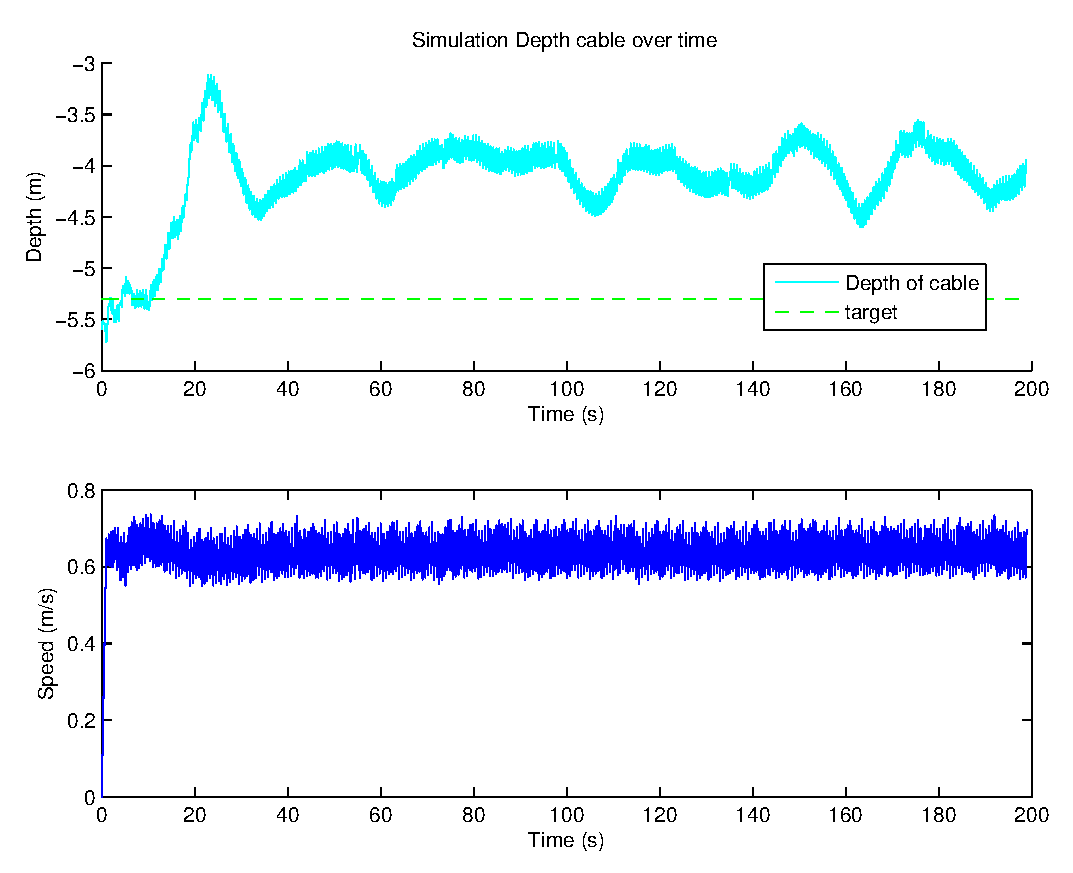
\includegraphics[scale=0.45,angle=0]{depth_controller_speed_rudder_sail_algo1}
    \caption{Depth and speed of the boat under algorithm~\ref{alg:breakAlg1}.}
    \label{fig: algo1Depth}
    \end{minipage}
    \hfill
    \begin{minipage}[b]{0.45\textwidth}
    \centering
    \includegraphics[scale=0.45,angle=0]{depth_controller_path_rudder_sail_algo1}
    \caption{Path of the boat under algorithm~\ref{alg:breakAlg1}.}
    \label{fig:algo1Path}
    \end{minipage}
\end{figure}
 
Using the rudder to slow down the boat is does not seem to be an efficient idea as seen in~\ref{fig:algo1Path} the boat is not following the line exactly around 5 meters off the line (initial condition is the boat is directly on the right path and downwind. The speed is also not steady and fluctuate a lot during the run.

 Then the test can be done with only controlling the sail for managing the speed here a PID controller:


\begin{algorithm}[H]
\caption{PID Speed sailbot controller using sail only}
\label{alg:breakAlg2}
\begin{algorithmic}[1]
\REQUIRE $v_{target}$, $v_{boat}$\\
   $\delta_s$ : Sail command given by conventional navigation algorithm\\
   $\delta_r$ : Rudder command given by conventional navigation algorithm\\
   $K_D$ : derivative coefficient for the PID controller $ K_D < 0$\\
   $K_I$ : integral coefficient for the PID controller $ K_I < 0$\\
\STATE $\Delta_{v} \leftarrow v_{target} - v_{boat}$
\IF{$\Delta_{v} \leq  0 $}
\STATE $\delta_s \leftarrow 0$
\ELSE
\IF{$v_{boat} > 0$}
\STATE $\delta_s \leftarrow \delta_s \cdot (\frac{\Delta_v}{v_{target}} + K_D \cdot \dot{\Delta}_v + K_I \cdot \displaystyle \int \Delta_v )$
\ENDIF
\ENDIF
\end{algorithmic}
\end{algorithm}

\begin{figure}[H]
\centering
    \begin{minipage}[b]{0.4\textwidth}
    \centering
    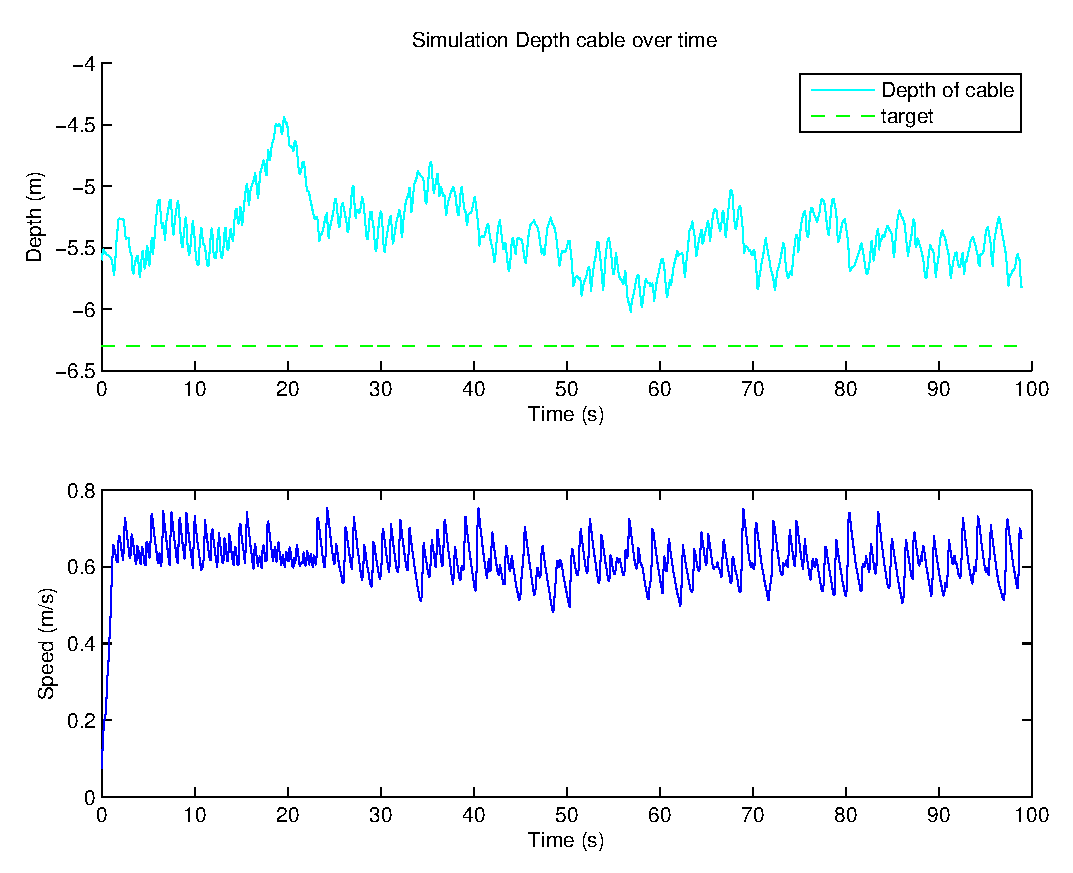
\includegraphics[scale=0.45,angle=0]{depth_controller_speed_rudder_sail_algo2}
    \caption{Depth and speed of the boat under algorithm~\ref{alg:breakAlg1}.}
    \label{fig: algo2Depth}
    \end{minipage}
    \hfill
    \begin{minipage}[b]{0.45\textwidth}
    \centering
    \includegraphics[scale=0.45,angle=0]{depth_controller_path_rudder_sail_algo2}
    \caption{Path of the boat under algorithm~\ref{alg:breakAlg1}.}
    \label{fig:algo2Path}
    \end{minipage}
\end{figure}

The PID controller does not completely solve the problem of the algorithm~\ref{alg:breakAlg1}, the error of the path taken by the boat is reduced but it still seems to have an offset (~\ref{fig:algo2Path}). This also induce oscillation on the cable that may not be good for the measurement on a survey.

The following algorithm is a modified version of a proportional controller as there is no derivative or integral term but the output is not, see~\ref{fig:responAlgo3} for the profile of the sail command depending on the speed error.

\begin{figure}[H]
\centering
    \begin{minipage}[b]{0.4\textwidth}
    \begin{algorithm}[H]
\caption{Speed sailbot controller using sail only}
\label{alg:breakAlg3}
\begin{algorithmic}[1]
\REQUIRE $v_{target}$, $v_{boat}$\\
   $\delta_s$ : Sail command\\
   $\delta_r$ : Rudder command\\
   $k$ : coefficient $(0< k <1)$\\
\STATE $\Delta_{v} \leftarrow v_{target} - v_{boat}$
\IF{$\Delta_{v} \leq  0 $}
\STATE $\delta_s \leftarrow 0$
\ELSE
\STATE $\delta_s \leftarrow \delta_s \cdot  \exp(-k \cdot (\frac{v_{target}}{\Delta_v}-1)) $
\ENDIF
\end{algorithmic}
\end{algorithm}
    \end{minipage}
    \hfill
    \begin{minipage}[b]{0.45\textwidth}
    \centering
    \includegraphics[scale=0.45,angle=0]{response_algo3}
    \caption{Value of the sail angle multiplier depending on the speed error }
    \label{fig:responAlgo3}
    \end{minipage}
\end{figure}




\begin{figure}[H]
\centering
    \begin{minipage}[b]{0.4\textwidth}
    \centering
    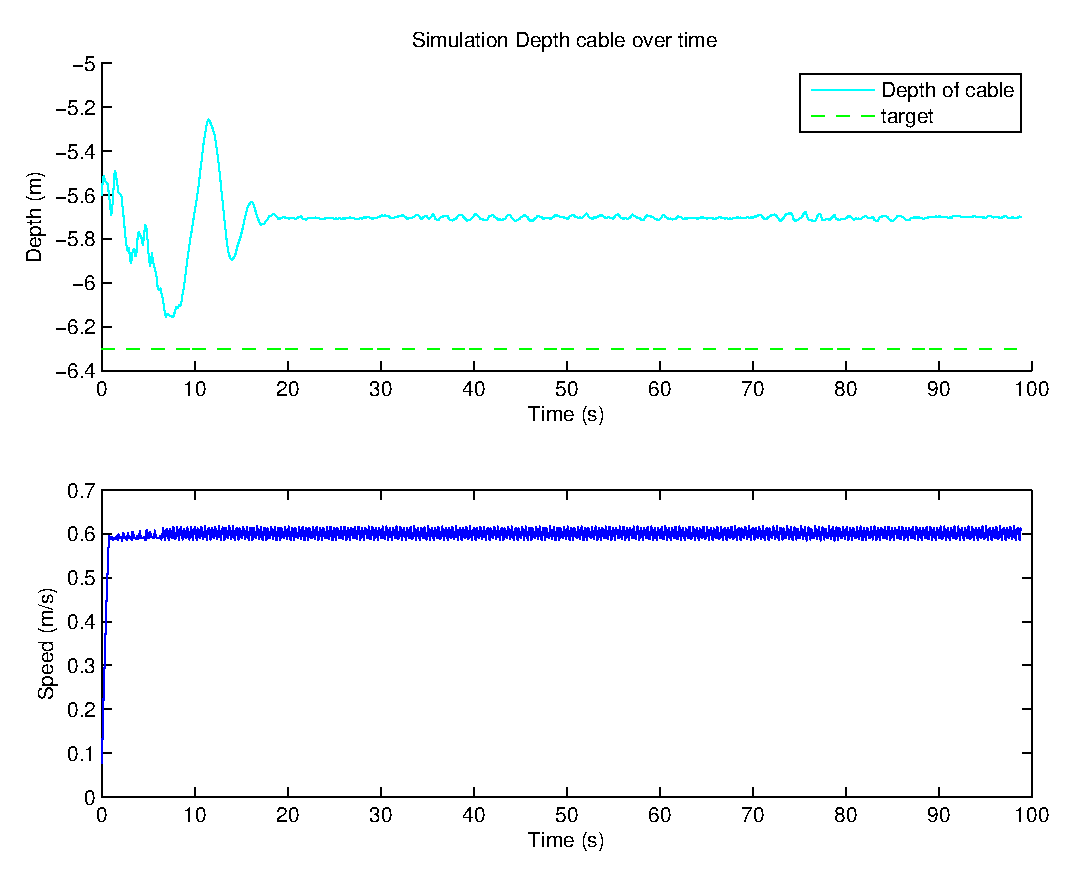
\includegraphics[scale=0.45,angle=0]{depth_controller_speed_rudder_sail_algo3}
    \caption{Depth and speed of the boat under algorithm~\ref{alg:breakAlg1}.}
    \label{fig: algo3Depth}
    \end{minipage}
    \hfill
    \begin{minipage}[b]{0.45\textwidth}
    \centering
    \includegraphics[scale=0.45,angle=0]{depth_controller_path_rudder_sail_algo3}
    \caption{Path of the boat under algorithm~\ref{alg:breakAlg1}.}
    \label{fig:algo3Path}
    \end{minipage}
\end{figure}

The algorithm~\ref{alg:breakAlg3} seems to be working on simulation, but suppose that when $\delta_s = 0$ the wind does not have any effect on the boat. But in general the main sail in itself is not rigid therefore the wind will still have an effect on the boat. They also have a front sail which is not controlled and will make the boat go forward. If these two non controllable forces are more powerful than the friction of the water then the boat will not be able to slow down to the right speed with only the control of the sail.

A solution to resolve this problem would to put weight on the cable so that the minimal speed increases (see~\ref{fig:depth_length_speed_pendulum}), adding length to the cable would not help on normal speed superior to 1 meter per second.


Another solution would be to add to the boat a device that would counter the effect of the front sail and the remaining of the main sail. Something simple as board placed to slow down , the surface of this board could be computed to match the push created by the sails.
 
A more advance solution would be to have controllable flap as some foiling boat could have but without  making the boat go up or down. The effect need to be symmetric to the horizontal line :

\begin{figure}[H]
\centering
\psscalebox{0.5 0.5} % Change this value to rescale the drawing.
{
% \usepackage[usenames,dvipsnames]{pstricks}
% \usepackage{epsfig}
% \usepackage{pst-grad} % For gradients
% \usepackage{pst-plot} % For axes
% \usepackage[space]{grffile} % For spaces in paths
% \usepackage{etoolbox} % For spaces in paths
% \makeatletter % For spaces in paths
% \patchcmd\Gread@eps{\@inputcheck#1 }{\@inputcheck"#1"\relax}{}{}
% \makeatother
% % User Packages:
% \usepackage{amsmath}
% \usepackage{amsfonts}
% \usepackage{amssymb}
% \usepackage{algorithm}
% \usepackage{algorithmic}
% 
\psscalebox{1.0 1.0} % Change this value to rescale the drawing.
{
\begin{pspicture}(0,-2.594394)(13.178725,2.594394)
\psline[linecolor=black, linewidth=0.04](0.01,-1.21312)(13.178696,-1.2357286)
\psline[linecolor=black, linewidth=0.04](6.599347,2.5943327)(6.5893474,-1.2556674)
\psframe[linecolor=black, linewidth=0.04, dimen=outer](3.23,0.16560608)(0.0,-1.2043939)
\psframe[linecolor=black, linewidth=0.04, dimen=outer](6.42,-1.214394)(3.19,-2.584394)
\psframe[linecolor=black, linewidth=0.04, dimen=outer](9.97,-1.224394)(6.74,-2.594394)
\psframe[linecolor=black, linewidth=0.04, dimen=outer](13.16,0.12560607)(9.93,-1.244394)
\rput[bl](4.49,1.785606){{\Large Flap} }
\psline[linecolor=black, linewidth=0.02, arrowsize=0.05291667cm 2.0,arrowlength=1.4,arrowinset=0.0]{->}(4.4,1.6856061)(2.5,0.38560608)
\psline[linecolor=black, linewidth=0.02, arrowsize=0.05291667cm 2.0,arrowlength=1.4,arrowinset=0.0]{->}(4.84,1.4756061)(4.66,-0.9243939)
\psline[linecolor=black, linewidth=0.02, arrowsize=0.05291667cm 2.0,arrowlength=1.4,arrowinset=0.0]{->}(5.68,1.6156061)(8.03,-1.0043939)
\psline[linecolor=black, linewidth=0.02, arrowsize=0.05291667cm 2.0,arrowlength=1.4,arrowinset=0.0]{->}(6.01,1.9256061)(9.61,-0.20439392)
\end{pspicture}
}


}
\caption*{Example of manipulable flap to put under the boat.}
\label{fig:model_boat_}
\end{figure}

